%
% $RCSfile: scalability.tex,v $
%
% Copyright (C) 2002-2008. Christian Heller.
%
% Permission is granted to copy, distribute and/or modify this document
% under the terms of the GNU Free Documentation License, Version 1.1 or
% any later version published by the Free Software Foundation; with no
% Invariant Sections, with no Front-Cover Texts and with no Back-Cover
% Texts. A copy of the license is included in the section entitled
% "GNU Free Documentation License".
%
% http://www.cybop.net
% - Cybernetics Oriented Programming -
%
% http://www.resmedicinae.org
% - Information in Medicine -
%
% Version: $Revision: 1.1 $ $Date: 2008-08-19 20:41:08 $ $Author: christian $
% Authors: Christian Heller <christian.heller@tuxtax.de>
%

\section{Scalability}
\label{scalability_heading}
\index{Scalability}
\index{Vertical Scaling}
\index{Horizontal Scaling}
\index{Symmetric Multiprocessing}
\index{SMP}
\index{Central Processing Units}
\index{CPU}
\index{Operating System}
\index{OS}
\index{Input/ Output}
\index{i/o}
\index{Reliability, Availability, Serviceability}
\index{RAS}
\index{Clustering}
\index{Vertical System}
\index{Horizontal System}
\index{Large Database}
\index{Web Server}
\index{Transactional Database}
\index{Firewall}
\index{Data Warehouse}
\index{Proxy Server}
\index{Data Mining}
\index{Directories}
\index{Application Server}
\index{High Performance Technical Computing}
\index{HPTC}
\index{Media Streaming}
\index{Extensible Markup Language Processing}
\index{XML}
\index{Java Server Pages Application}
\index{JSP}
\index{Secure Socket Layer}
\index{SSL}
\index{Virtual Private Network}
\index{VPN}
\index{Application Types}
\index{Interconnect}
\index{Loosely-coupled external Interconnect}
\index{Tightly-coupled internal Interconnect}

The previous sections demonstrated that there are many different ways to organise
a distributed information technology environment. The physical distribution of
systems is often a user requirement, either to connect different locations or to
reach better performance by sharing the work load. The degree to which a system
can be distributed to different hardware is often called its \emph{Scalability}.
Two models of scaling can be distinguished: \emph{vertical} and \emph{horizontal}
computing (figure \ref{scaling_figure}), whose key characteristics are only
described briefly here.

\begin{figure}[ht]
    \begin{center}
        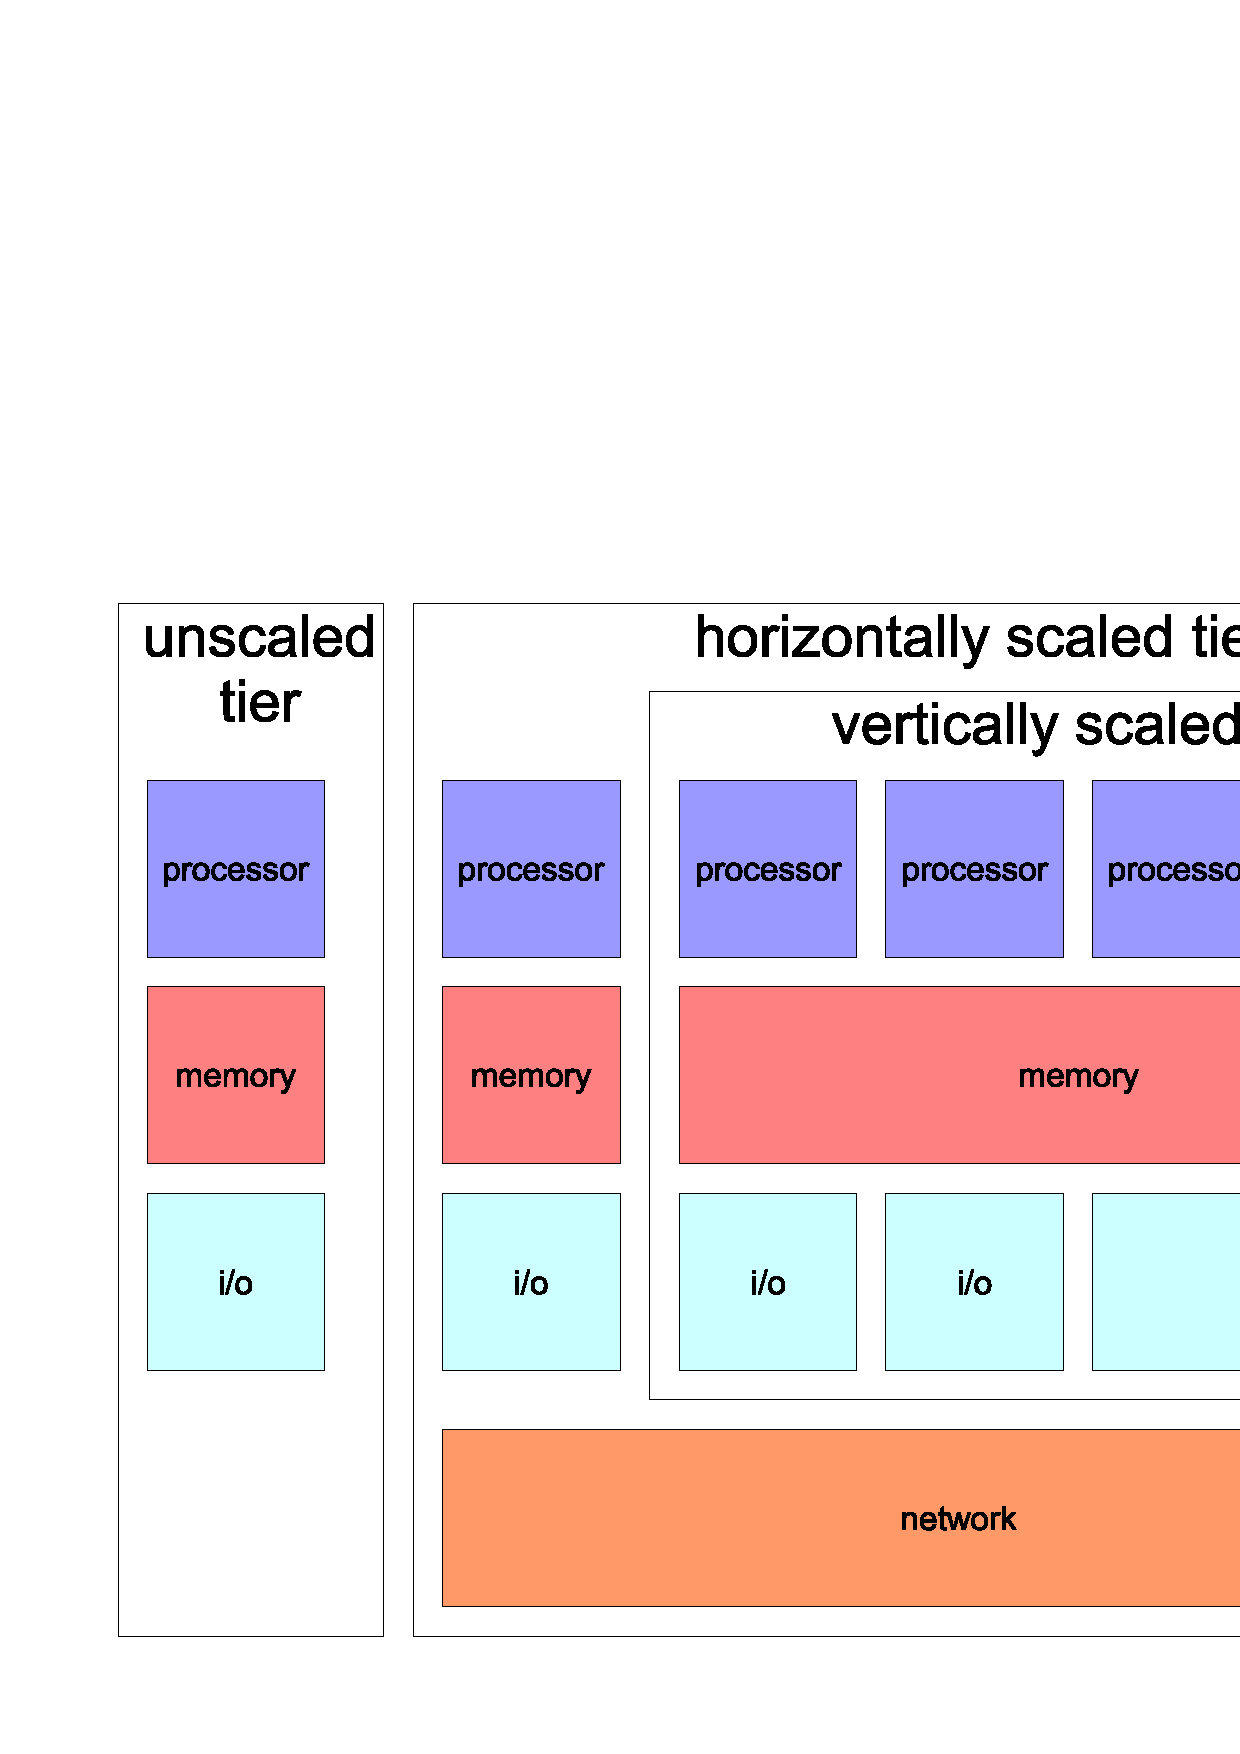
\includegraphics[scale=0.3,angle=-90]{graphic/scaling.pdf}
        \caption{Vertical and Horizontal Scaling}
        \label{scaling_figure}
    \end{center}
\end{figure}

Vertical servers are large \emph{Symmetric Multiprocessing} (SMP) systems with
more than four \emph{Central Processing Units} (CPU) that share one common memory.
One single \emph{Operating System} (OS) instance covers the processors, the memory
and input/ output (i/o) components. Vertical servers provide high availability by
building numerous \emph{Reliability, Availability, Serviceability} (RAS) features
into the individual server, to minimise un-/planned downtime.

The alternative horizontal scaling connects many systems over network, which is
often called \emph{Clustering}. A cluster contains computing nodes having one to
four processors and a memory each. The input/ output devices may belong to just
one node or be shared by many. Each node has an OS instance. \textit{Horizontal
servers do not build RAS features into the individual servers but get high RAS
by replication and deployment of many servers}, as Atwood \cite{atwood} writes.

\begin{table}[ht]
    \begin{center}
        \begin{footnotesize}
        \begin{tabular}{| p{50mm} | p{60mm} |}
            \hline
            \textbf{Vertical System} & \textbf{Horizontal System}\\
            \hline
            Large Database & Web Server\\
            \hline
            Transactional Database & Firewall\\
            \hline
            Data Warehouse & Proxy Server\\
            \hline
            Data Mining & Directories\\
            \hline
            Application Server & Application Server\\
            \hline
            High Performance Technical Computing (HPTC) application (non-partitionable) & High Performance Technical Computing (HPTC) application (partitionable)\\
            \hline
            & Media Streaming\\
            \hline
            & Extensible Markup Language (XML) Processing\\
            \hline
            & Java Server Pages (JSP) Application\\
            \hline
            & Secure Socket Layer (SSL)\\
            \hline
            & Virtual Private Network (VPN)\\
            \hline
        \end{tabular}
        \end{footnotesize}
        \caption{Vertical and Horizontal Application Types \cite{atwood}}
        \label{scalability_table}
    \end{center}
\end{table}

Table \ref{scalability_table} states some typical applications for vertical and
horizontal computing. The key difference, that after \cite{atwood} affected
both, their price and performance, is the \emph{Interconnect} used with each
architecture. Horizontal servers use a loosely-coupled \emph{external}
interconnect. Vertical servers use a tightly-coupled \emph{internal}
interconnect that makes data communications faster.
